In this chapter we describe our tools \coconet{} and \nevertwo{} that
are part of the \textit{NeVerTools} suite. The two tools are complementary 
and serve two purposes: \coconet{} aims to bridge the gap between the 
representation and the conversion of neural networks in the verification 
community; on the other hand, \nevertwo{} is our graphical user interface 
(GUI) for learning and verification.
Both \coconet{} and \nevertwo{} are written in Python and rely on two components:
the \pynever{} API~\cite{guidotti2021pynever} which contains the actual methods 
for the training and verification and the PyQt5 API~\cite{summerfield2007rapid}
which allows to design GUIs for a desktop environment.

\section{\coconet{}}
\label{sec:coconet}

The verification community has stabilized in the recent years and started in
2020 the International Verification of Neural Networks Competition
(VNN-COMP)~\cite{muller2022third} that gathers verification
benchmarks for evaluating the performances of verification tools. In order
to even the workflow and process of verification tools, the VNN-COMP relies
on the VNN-LIB~\cite{vnnlib} standard, which consists of the ONNX~\cite{onnx}
file format for the neural networks and the SMT-LIB~\cite{smtlib} for the
specification of the property. Since there exist many different formats for
the representation of neural networks, we developed 
\coconet{}~\footnote{https://github.com/NeVerTools/CoCoNet} for allowing
researchers to convert their networks to ONNX. It is also possible to build a
network from scratch visually in the environment.

\subsection{Software architecture}

\begin{figure}[t]
	\caption{\label{fig:cd_coconet} UML Class Diagram representing the main
		software components of \coconet. Using the PyQt API we leverage the
		\texttt{QGraphicsView} and \texttt{QGraphicsScene} interfaces to build
		a workspace in the \texttt{QMainWindow}. On the other hand, the class
		\texttt{Scene} serves as a controller for the creation and display of
		graphics blocks and as an interface to the \pynever{} components.}
	\centering
	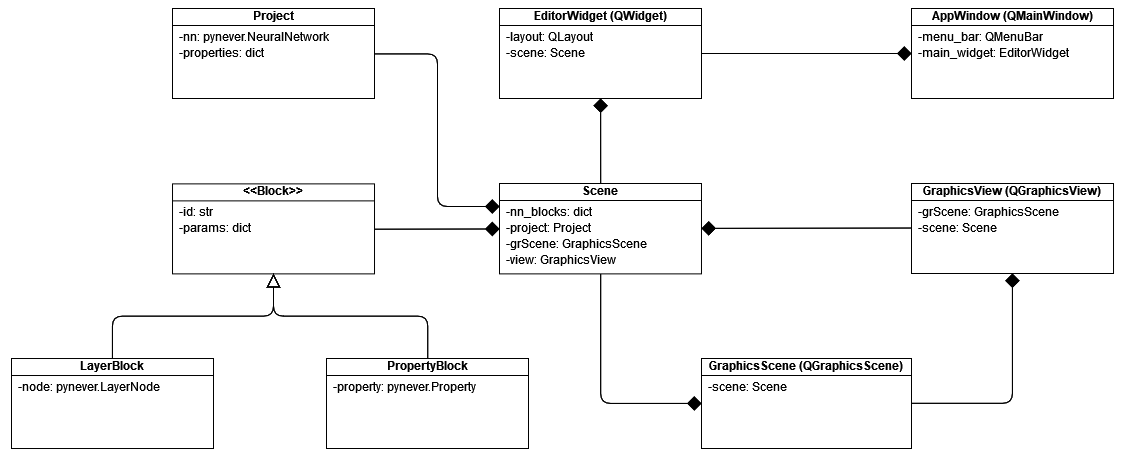
\includegraphics[width=\linewidth]{NN/CoCoNetCD.png}
\end{figure}

The architecture of \coconet{} is detailed in Figure~\ref{fig:cd_coconet}. Relying
on PyQt5's model for building GUIs, we use the classes \texttt{GraphicsScene} and
\texttt{GraphicsView} to control the logical model and the rendering, respectively.
In particular, we separate the building elements (blocks and edges) in the class
\texttt{Scene} from the methods and utilities for managing the exchange with the
view in \texttt{GraphicsScene}. The class \texttt{Project} serves as a
controller for reflecting the actions taken in the graphical environment to the
neural network that is built within \pynever. The main window of the application is 
displayed by the class \texttt{EditorWidget} which is associated with the 
\texttt{CoCoNetWindow} class containing the logic for displaying the 
\texttt{GraphicsView} and all the menus and layouts involved.

In order to comply with the VNN-LIB standard we have two kinds of available blocks:
the \texttt{LayerBlock} that represent the layers of a neural network, and the
\texttt{PropertyBlock} that represent a property to link to the input or the output
of the network. Each \texttt{LayerBlock} is initialized with a \texttt{LayerNode}
object from \pynever, i.e., represents a layer of the neural network displaying
all the fields and allowing the modification of some parameters. \texttt{PropertyBlock}
objects are initialized with a \pynever{} property, which allows to define a SMT-based
rule on the input and/or the output.

\subsection{Application interface}

\begin{figure}[t]
	\caption{\label{fig:coconet_gui} Screenshot of \coconet's GUI. The network
		is displayed in the Graphics Scene, and there is a toolbar with the 
		available blocks divided in nodes and properties on the left.}
	\centering
	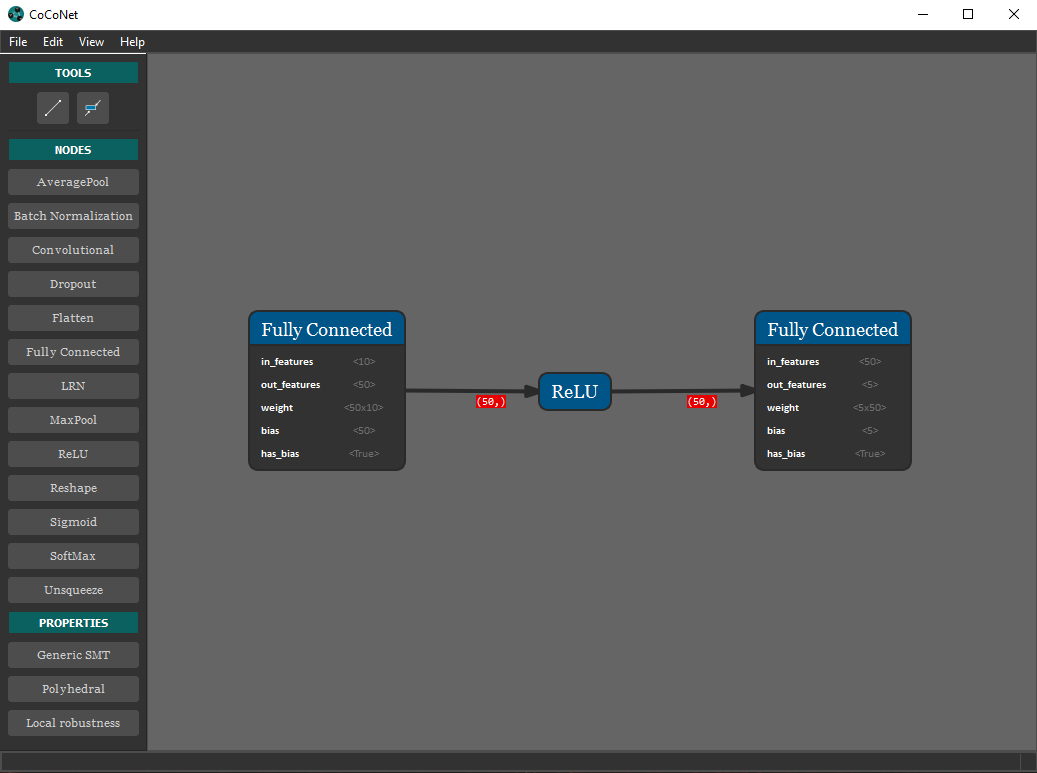
\includegraphics[width=.8\linewidth]{NN/CoCoNet_net.png}
\end{figure}

Figure~\ref{fig:coconet_gui} is a screenshot of \coconet's main window. The
view contains a simple network with a single Fully Connected layer with a ReLU
activation function. The available layers from \pynever{} are displayed in the
left toolbar, where the last three entries are different versions of a property.
The displayed nodes show the information related to the corresponding node: while
the ReLU layer has no parameters, the Fully Connected layer shows the inputs, the
outputs and the dimension of the weight and bias matrices. When a network is loaded
or created in the view, it is possible to add properties or save it in the VNN-LIB
format creating one ONNX file for the network and a SMT-LIB file for the property.

It is possible to connect one or more properties to the neural network displayed,
in the left toolbar we have three alternatives:
\begin{itemize}
	\item \textit{Generic SMT} - a simple text dialog where it is possible to directly
		write a property in plain SMT-LIB language
	\item \textit{Polyhedral} - a property that allows to set an upper or lower bound
		to each variable the property is connected to
	\item \textit{Local robustness} - a property that allows to specify a pair of
		input and output samples with an $\epsilon$-$\delta$ perturbation
\end{itemize}
%
\begin{figure}[t]
	\centering
	\caption{\label{fig:properties} Screenshot of the edit dialogs for three properties
		available in \coconet. From left to right, as described in the dialog label, 
		there is the \textit{Generic SMT} property, the \textit{Polyhedral} property 
		and the \textit{Local robustness} property.}
	\begin{subfigure}{.3\linewidth}
		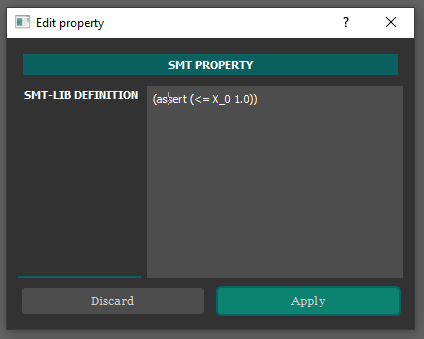
\includegraphics[width=\linewidth]{NN/Generic.png}
	\end{subfigure}
	\hspace*{\fill}
	\begin{subfigure}{.3\linewidth}
		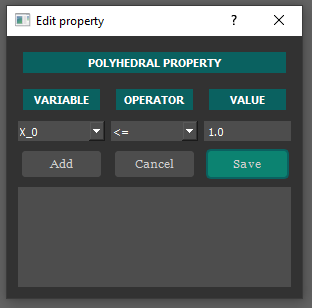
\includegraphics[width=\linewidth]{NN/Poly.png}
	\end{subfigure}
	\hspace*{\fill}
	\begin{subfigure}{.3\linewidth}
		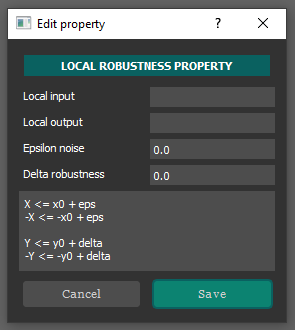
\includegraphics[width=\linewidth]{NN/LocRob.png}
	\end{subfigure}
\end{figure}
%
In Figure~\ref{fig:properties} we show the dialogs for the specification of the different
properties. For the \textit{Polyhedral} property the variables are constrained to the
number of inputs for a \textit{pre}-condition or the number of outputs for a 
\textit{post}-condition and can be bounded with all the relational operators, i.e.,
$<, \leq, =, >, \geq$. The \textit{Local robustness} property requires two samples, one
for the input and one for the output, and the two $\epsilon$ and $\delta$ measures.

Once the network and the properties are set, it is possible to save the benchmark in the
VNN-LIB format: using the \textit{Save as...} menu, it is possible to select 
\textit{VNN-LIB} as the output file format. In this way, the neural network will be saved
--- or converted, if opened as a different format --- as an ONNX file and the properties
will be stored in a separate SMT-LIB file with the same name of the network.